% Figure 3.5 (Session 3): spin-charge separation in the half-filled Hubbard chain.
% The image is rendered by figures/blender/s3_5_spin_charge.py; the coordinates of the labels
% come from figures/blender/out/spin_charge_anchors.tex. Compile with:
%   pdflatex spin_charge.tex ; result moves to ../many_body_fermions/spin_charge.pdf
\documentclass[11pt,tikz,border=0pt]{standalone}
\usepackage{amsmath,amssymb,graphicx}
\usepackage{xcolor}
\definecolor{coursedark}{HTML}{1B2A4A}
\definecolor{costamber}{HTML}{B8620A}
\newlength{\figw}\setlength{\figw}{16.19cm}   % the text width of the notes (letter, 2.7 cm margins), so labels print at size

\begin{document}
\begin{tikzpicture}[lbl/.style={font=\small, text=coursedark}]
  \node[anchor=south west, inner sep=0pt] at (0,0)
    {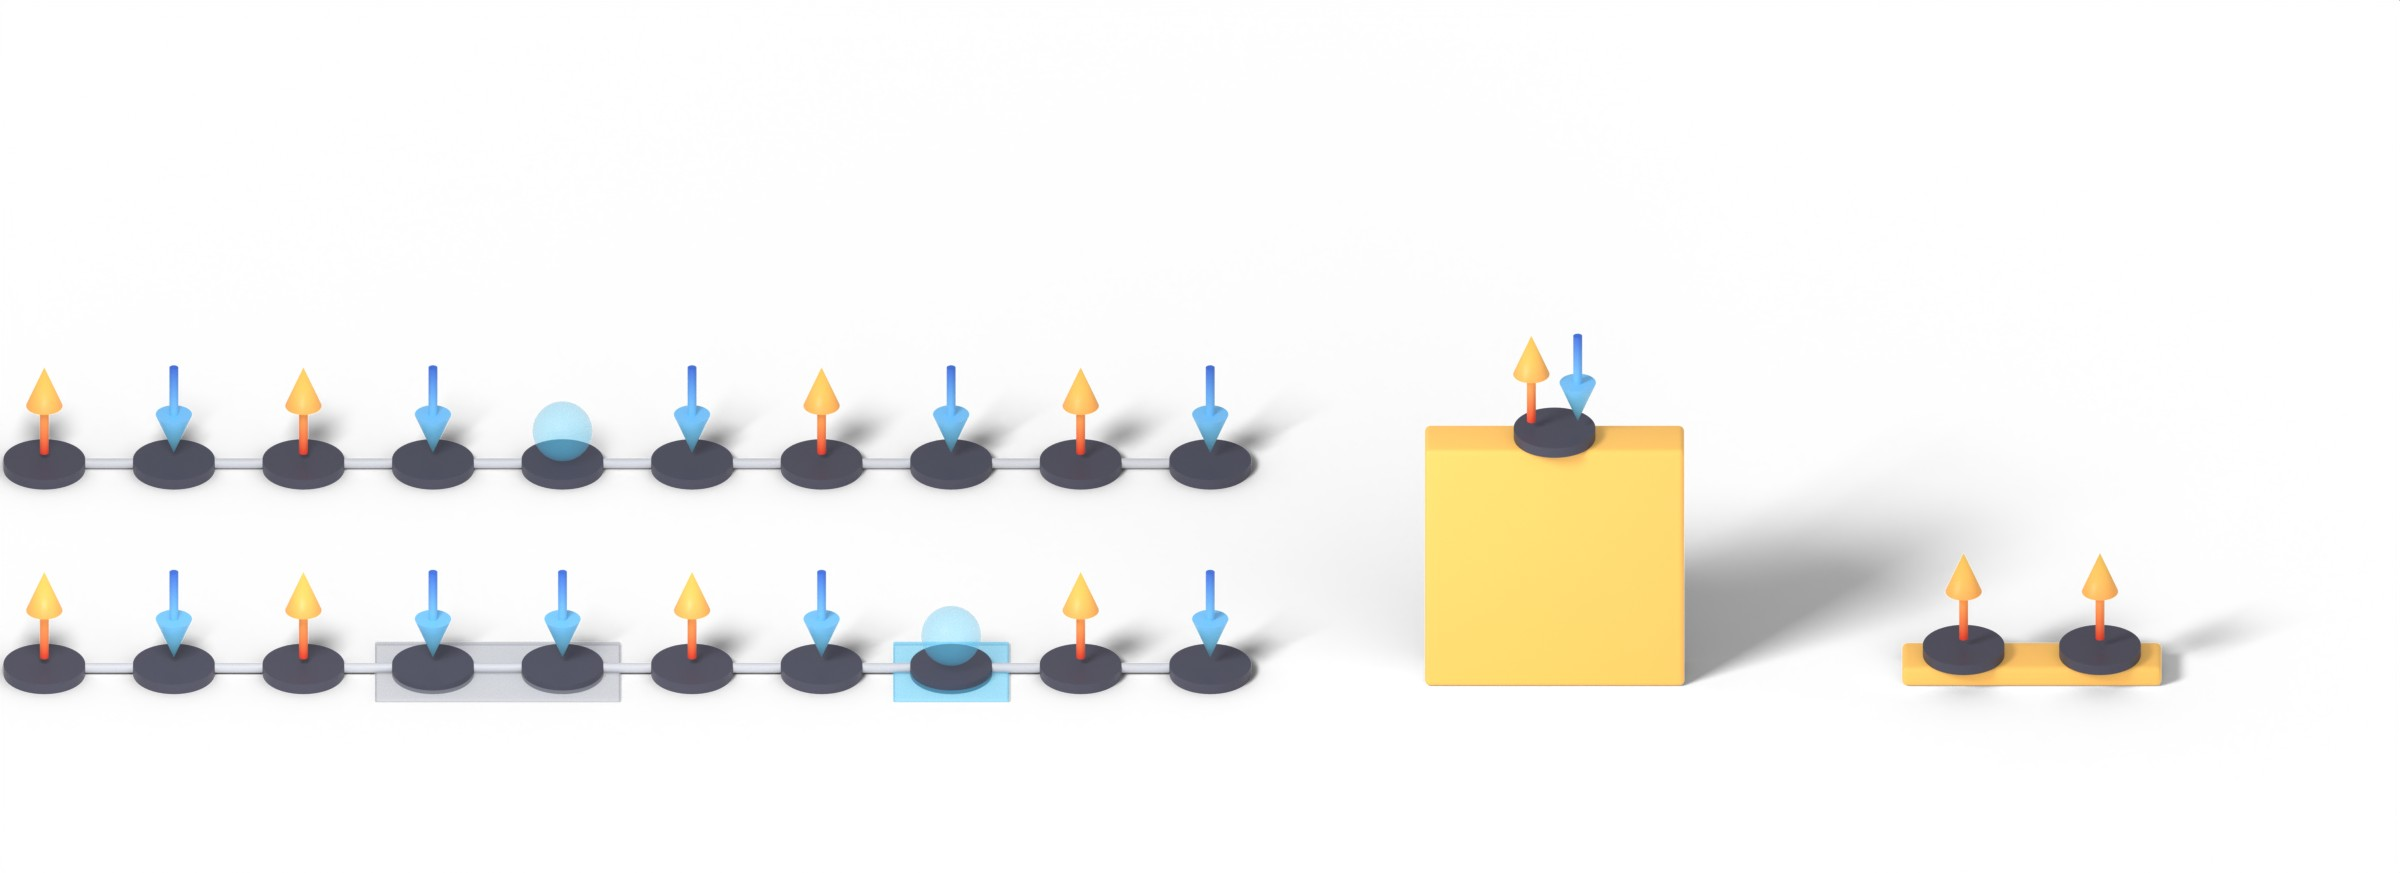
\includegraphics[width=\figw]{../blender/out/spin_charge.jpg}};
  %% written by figlib.py; x and y in units of the image width
\coordinate (removed) at (0.2344\figw,0.2165\figw);
\coordinate (holon) at (0.3963\figw,0.0617\figw);
\coordinate (spinon) at (0.2074\figw,0.0617\figw);
\coordinate (a) at (0.0028\figw,0.2815\figw);
\coordinate (U) at (0.6477\figw,0.0660\figw);
\coordinate (J) at (0.8466\figw,0.0660\figw);
\coordinate (b) at (0.5455\figw,0.2815\figw);

  \node[lbl, font=\normalsize, anchor=west] at (a) {(a)};
  \node[lbl, font=\normalsize, anchor=west] at (b) {(b)};
  \node[lbl, anchor=south] at (removed) {electron removed};
  \node[lbl, anchor=north] at (spinon) {spinon};
  \node[lbl, anchor=north] at (holon) {holon};
  \node[lbl, anchor=north, text=costamber, align=center] at (U) {added electron,\\a doublon, $\approx U/2$};
  \node[lbl, anchor=north, text=costamber, align=center] at (J) {spin flip\\$\approx J=4t^2/U$};
\end{tikzpicture}
\end{document}
